%=======================02-713 LaTeX template, following the 15-210 template==================
%
% You don't need to use LaTeX or this template, but you must turn your homework in as
% a typeset PDF somehow.
%
% How to use:
%    1. Update your information in section "A" below
%    2. Write your answers in section "B" below. Precede answers for all 
%       parts of a question with the command "\question{n}{desc}" where n is
%       the question number and "desc" is a short, one-line description of 
%       the problem. There is no need to restate the problem.
%    3. If a question has multiple parts, precede the answer to part x with the
%       command "\part{x}".
%    4. If a problem asks you to design an algorithm, use the commands
%       \algorithm, \correctness, \runtime to precede your discussion of the 
%       description of the algorithm, its correctness, and its running time, respectively.
%    5. You can include graphics by using the command \includegraphics{FILENAME}
%
\documentclass[11pt]{article}
\usepackage{amsmath,amssymb,amsthm}
\usepackage{graphicx}
\usepackage[margin=1in]{geometry}
\usepackage{fancyhdr}
\setlength{\parindent}{0pt}
\setlength{\parskip}{5pt plus 1pt}
\setlength{\headheight}{13.6pt}
\newcommand\question[2]{\vspace{.25in}\hrule\textbf{#1: } #2\vspace{.5em}\hrule\vspace{.10in}}
\renewcommand\part[1]{\vspace{.10in}\textbf{(#1)}}
\newcommand\runtime{\vspace{.10in}\textbf{Running time: }}
\pagestyle{fancyplain}
\lhead{\textbf{\NAME\ (\ANDREWID)}}
\chead{\textbf{Foundations of Finance HW\HWNUM}}
\rhead{\today}
\begin{document}\raggedright
%Section A==============Change the values below to match your information==================
\newcommand\NAME{Ramel Tranquille}  % your name
\newcommand\ANDREWID{rt1734}     % your andrew id
\newcommand\HWNUM{2}              % the homework number
%Section B==============Put your answers to the questions below here=======================

% no need to restate the problem --- the graders know which problem is which,
% but replacing "The First Problem" with a short phrase will help you remember
% which problem this is when you read over your homeworks to study.

\section{Portfolio Theory with 2 Risky Assets}
\question{1a}{Expected Return \& Standard Deviation} 

\begin{table}[h]
    \label{tab:}
    \begin{center}
        \begin{tabular}[c]{l|l|l}
            \hline
            \multicolumn{1}{c}{\textbf{  }} & 
            \multicolumn{1}{c}{\textbf{Security Y}} &
            \multicolumn{1}{c}{\textbf{Security X}} \\
            \hline
            Expected Return & 15\% & 35\% \\
            Expected Return & 20\% & 40\% \\
            Correlation & 0.25 \\
            
            \hline
        \end{tabular}
    \end{center}
\end{table}

Calculating the $E(R)$ and $\sigma$ from 1 to 5 with respective weights, $w_1$.\\ 
$$
    E(R) = w_1 E(R_1) + w_2 E(R_2)
$$
\[
    Var = \sigma^2_p = w^2_1 \sigma^2_1 + w^2_2 \sigma^2_2 + 2w_1w_2\sigma_1 \sigma_2 \rho
\]

\begin{table}[h]
    \begin{center}
        \begin{tabular}[c]{l|l|l}
            \hline
            \multicolumn{1}{c}{\textbf{  }} & 
            \multicolumn{1}{c}{\textbf{E(R)}} &
            \multicolumn{1}{c}{\textbf{$\sigma$}} \\
            \hline
            \textbf1. & .15\% & .200\% \\
            \textbf2. & .20\% & .200\% \\
            \textbf3. & .25\% & .245\% \\
            \textbf4. & .30\% & .316\% \\
            \textbf5. & .35\% & .400\% \\
            \hline
        \end{tabular}
    \end{center}
\end{table}

\question{1b}{Efficient Frontier Plot}
\begin{center}
    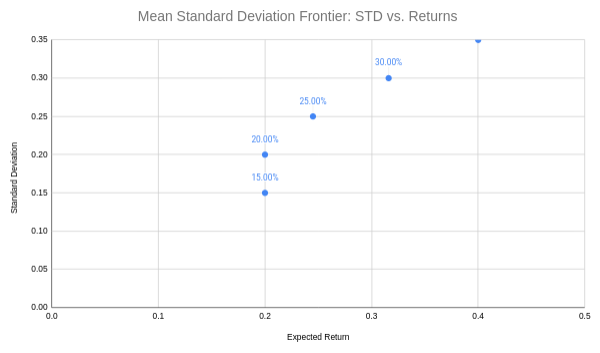
\includegraphics[width=10cm, height=6cm]{MeanSTD_Frontier}
\end{center}

\question{1c}{Efficient Portfolio}
Efficient portfolios which maximize the $E(R)$ (mean) and lowers the variation and standard deviation include 2-5.
Since, 2 and 1 have the same standard deviation, we accept the portfolio with the higher $E(R)$, 2.


\section{Portfolio Theory with a Riskless Asset}
\begin{itemize}
    \item $E(R) = 16\% \text{ and } \sigma = 10\%$
    \item $R_f = 8\%$
\end{itemize}

\question{2a}{Expected Return and Standard Deviation} 
Since the asset is risk free, the standard deviation of the portfolio is 0.
\question{2b}{50\% Weight in SnP}
$$
    E(R) = w_1 E(R_1) + w_2 E(R_2) = .5(.16) + .5(.08) = .08 + .04 = .12
$$ 
$$
    \sigma_p = w_M \sigma_M = (.5)(.10) = .05
$$ 

\question{2c}{Borrowing}
Portfolio with 125\% in SnP, with 25\% borrowed at risk-free asset rate.
\[
    \sigma = w_M \sigma_M = 1.25(.1) = 0.125 
\]
\[
    E(R) = w_m E(R_m) + w_{-m}E(R_f) = 1.25(.16) + -.25(.08) = .18
\]
Note: total weight cannot exceed 1

\question{2d}{Backwards Solving for Weight} 
We substitute $2\sigma_p$ for $\sigma_M$ and $w_M=-1$ so total weight $=1$. Thus,
$$
    2\sigma_M = w_M \sigma_M \rightarrow w_M = 2
$$
$$
    \sigma_p = w_m \sigma_m = 2(.10) = .2
$$
$$
    E(R) = w_fR_f + w_M R_M = -1(.08) + 2(.16) = .24
$$
\question{3}{Preference w/ T-Bill} 
\begin{table}[h]
    \begin{center}
        \begin{tabular}[c]{l|l|l}
            \hline
            \multicolumn{1}{c}{\textbf{  }} & 
            \multicolumn{1}{c}{\textbf{$E(R)$}} &
            \multicolumn{1}{c}{\textbf{$\sigma$}} \\
            \hline
            Russel Fund & .16 & .12 \\
            Windsor Fund & .14 & .10 \\
            SnP Fund & .12 & .08 \\
            \hline
        \end{tabular}
    \end{center}
\end{table}

\begin{itemize}
    \item Russel Fund
    \item Windsor Fund
    \item SnP Fund
    \item $0.6 = w_R$ and $0.4 = w_{snp}$
\end{itemize}

To find the best fund, we calculate the sharpe ratio with $R_t=0.6\%$:
\[
    \text{Russel} = \frac{E(R_r) - R_t}{\sigma_r} = \frac{.16-.06}{0.12} = 0.8333
\]

\[
    \text{Windsor} = \frac{E(R_w) - R_t}{\sigma_w} = \frac{.14-.06}{0.10} = 0.8
\]

\[
    \text{SnP} = \frac{E(R_{snp}) - R_t}{\sigma_{snp}} = \frac{.12-.06}{0.08} = 0.75
\]
Finding $E(R_M) \text{, } \sigma_M $ and the sharpe ratio. Note: $w_2 = \text{weight of SnP}$
\[
    E(\text{60/40}) = .6E(R_r) + .4E(R_{snp}) = .6(.16) + .4(.12) = .144
\]

\[
    \sigma^2_m = w^2_1 \sigma^2_1 + w^2_2 \sigma^2_2 + 2w_1w_2\sigma_1 \sigma_2 \rho 
\]
\[
    = (.36)(.0144)+(.16)(.0064)+2(.6)(.4)(.7)(.12)(.08)=0.0094336
\]

\[
    \sqrt{\sigma^2_m} = \sqrt{0.0094336} = 0.0971267213
\]

\[
    \text{sharpe-ratio} = \frac{E(R_M) - R_t}{\sigma_m} = \frac{0.144 - 0.6}{0.0971267213} = 0.8648495375
\]

Thus, we would choose the 60/40 Portfolio since it has the highest sharpe ratio.
\begin{table}[h]
    \begin{center}
        \begin{tabular}[c]{l|l|l|l}
            \hline
            \multicolumn{1}{c|}{\textbf{  }} & 
            \multicolumn{1}{c|}{\textbf{$E(R)$}} &
            \multicolumn{1}{c|}{\textbf{$\sigma$}} &
            \multicolumn{1}{c}{Sharpe Ratio} \\
            \hline
            Russel Fund & .16 & .12 & 0.8333\\
            Windsor Fund & .14 & .10 & 0.800\\
            SnP Fund & .12 & .08 & 0.750\\
            60/40 & .144 & .097 & 0.8648\\
            \hline
        \end{tabular}
    \end{center}
\end{table}


\pagebreak
\section{The Capital Asset Pricing Model (CAPM)}
\begin{itemize}
    \item $R_f = 0.04$
    \item $E(R_M) = .12$
    \item $\sigma_m = .15$
\end{itemize}
\question{4a}{Equilibrium Risk Premium} 
\[
    \text{ERP} = E(R_M) - R_f = 0.12 - 0.4 = .8
\]

\question{4b}{Realized Return \& Beta} 
We cannot compute the beta of this stock, because we are given realized return, not $E(R)$.

\question{4c}{Expected Return \& Beta} 
\[
    \beta = \frac{E(R)-R_f}{E(R_M)-R_f} = \frac{.15-.04}{.12-.04} = 1.25
\]
\end{document}
